\documentclass[thesis.tex]{subfiles}

\begin{document}

\iffulldocument\else
	\chapter{The 5th order KdV equation: $n$-homoclinic solutions}
\fi

A multi-pulse is a localized, multi-modal solution to \cref{eqODE} which resembles multiple, well-separated copies of the primary pulse. Heuristically, we construct a multi-pulse by gluing together multiple copies of the primary pulse end-to-end. This is shown in \cref{fig:multipulse}.
\begin{figure}
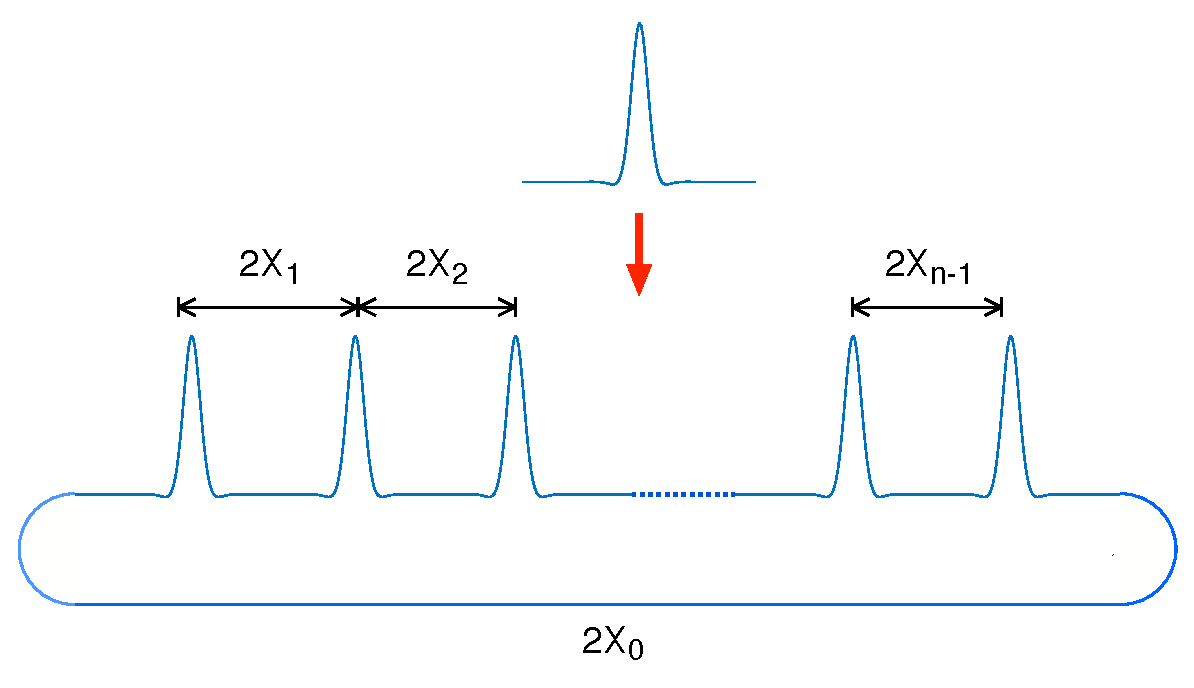
\includegraphics[width=12cm]{images/kdv5numerics/multipulseperiodic.eps}
\caption{Construction of an $n$-pulse solution from the primary pulse.}
\label{fig:multipulse}
\end{figure}

\noi In this chapter, we will discuss the existence and spectral stability of multi-pulses.

\section{Existence of multi-pulses}\label{sec:multiexistR}

First, we look at existence. From a spatial dynamics perspective, an $n$-pulse is a $n$-loop homoclinic orbit solution $Q_n(x)$ to
\begin{equation}\label{existgenODE1}
U'(x) = F(U(x); c)
\end{equation}
which remains close to the primary homoclinic orbit $Q_n(x)$. An $n$-pulse can be described by $n-1$ pulse distances $\{X_1, \dots, X_{n-1} \}$, where the distance between consecutive copies of $Q(x)$ is $2 X_j$.

From a mathematical perspective, rather than describing a $n$-pulse by its pulse distances $X_j$, we will use an alternative parameterization which more convenient and which captures the underlying geometry necessary for a multi-pulse to exist. This parameterization is almost identical to that in \cite{SandstedeStrut,Sandstede1998}.

From Hypothesis \ref{hypeqhyp}, the rest state at 0 is a hyperbolic equilibrium point of \cref{existgenODE}. The linearization $DF(0; c)$ about the rest state has a quartet of eigenvalues $\pm \alpha_0 \pm \beta_0 i$, which depends on the wavespeed $c$. All other eigenvalues have real part strictly larger in magnitude than $\alpha_0$. Let
\begin{equation*}
\rho = \frac{\beta_0}{\alpha_0},
\end{equation*}
and define the set
\begin{align*}
\mathcal{R} &= \left\{ \exp\left(-\frac{2 k \pi}{\rho}\right) : k \in \N_0 \right\} \cup \{ 0 \},
\end{align*}
which is a complete metric space. We will use $r \in \mathcal{R}$ as a scaling parameter. The parameterization works as follows.

\begin{definition}\label{def:homparam}
For $n \geq 2$, a \emph{homoclinic parameterization} of an $n$-pulse is a sequence of nonnegative integers $(m_1, \dots, m_{n-1}$, where at least one of the $m_j \in \{0, 1\}$.
\end{definition}
The pulse distances $X_j$ are determined from the integers $m_j$ and the scaling parameter $r$, as will be shown in the next theorem. The requirement that one of the $m_j$ must be 0 or 1 is necessary for a multi-pulse to be uniquely described by a homoclinic parameterization and a scaling parmeter $r$. The following theorem, which is adapted from \cite[Theorem 3.6]{SandstedeStrut}, gives an existence result for multi-pulse solutions.

\begin{theorem}[Existence of Multi-Pulses]\label{multipulseexistR}
Assume Hypotheses \ref{Ehyp}, \ref{Hhyp}, \ref{hypeqhyp}, \ref{Qexistshyp}, and \ref{H0transversehyp}. Let $Q(x)$ be the transversely constructed, symmetric primary pulse solution to \eqref{genODE} from Hypothesis \ref{Qexistshyp}. Then there exists $\delta > 0$ such that the following holds. For any homoclinic parameterization $(m_1, \dots, m_{n-1})$, there exists $r_* = r_*(m_1, \dots, m_{n-1}) \in \mathcal{R}$ with $r_* > 0$ such that for any $r \in \mathcal{R}$ with $r \leq r_*$:
\begin{enumerate}[(i)]
\item There exists a unique $n$-pulse solution $Q_n$ to \cref{genODE} which resembles $n$ consecutive copies of $Q$. 
\item The distances between consecutive copies of $Q(x)$ are $2 X_j(r)$, where
\begin{align}\label{nhompeaks}
X_j(r; m_j) &= \frac{1}{2 \alpha_0} |\log r| + \frac{1}{2\beta_0} t_j(r; m_j) + L_0 && j = 1, \dots, n-1
\end{align}
The $t_j(r; m_j): \mathcal{R} \rightarrow \R$ are smooth functions with $t_j(0; m_j) = m_j \pi$, and $L_0$ is a constant.

\item There are exactly $n$ real eigenvalues $\lambda_j$ of $\calE''(q_n)$ with $|\lambda_j| < \delta$. These are as follows.
\begin{enumerate}
	\item There are $n_{\text{odd}}$ negative eigenvalues, where $n_{\text{odd}}$ is the number of $m_j$ which are odd.
	\item There are $n_{\text{even}}$ positive eigenvalues, where $n_{\text{even}}$ is the number of $m_j$ which are even.
	\item There is a simple eigenvalue at 0 with corresponding eigenfunction $\partial_x Q_n$.
\end{enumerate}

\item We can write $Q_n(x)$ in piecewise form consisting of $2n$ pieces $\{ Q_j^\pm(x) : j = 1, \dots, n \}$, where $Q_j^-: [-X_{j-1}, 0] \rightarrow \R^{2m}$ and $Q_j^+: [0, X_j] \rightarrow \R^{2m}$, with $X_0 = X_n = \infty$. The pieces are joined together end-to-end as in \cite{Sandstede1998}. Each piece $Q_j^\pm(x)$ is a small perturbation of the primary pulse $Q(x)$ of the form
\begin{equation}\label{Qpmexpansions}
Q_j^\pm(x) = Q(x) + \tilde{Q}_j^\pm(x),
\end{equation}
where for the remainder terms $\tilde{Q}_j^\pm(x)$ we have the estimates
\begin{equation}\label{Qpmestimates}
\begin{aligned}
\|\tilde{Q}_j^\pm\| &\leq C e^{-\alpha_0 X_{\min}} \\
|\tilde{Q}_{j+1}^-(-X_j) - Q(X_j)| &\leq C e^{-2 \alpha_0 X_{\min}} \\
|\tilde{Q}_j^+(X_j) - Q(-X_j)| &\leq C e^{-2 \alpha_0 X_{\min}} \\
\end{aligned}
\end{equation}
which hold in addition for derivatives of $Q$.
\end{enumerate}
\begin{proof}
Parts (i)-(iii) follow from \cite{SandstedeStrut}, where $L_j(r)$ in \cite{SandstedeStrut} corresponds to $2X_j(r)$ here. \cref{hypeqhyp} and \cref{Hhyp} are equivalent to Hypotheses 3.1 and 3.3 in \cite{SandstedeStrut}. The eigenvalue problem $\calE''(q_n)v = \lambda v$ can be written in a first order system as
\[
V'(x) = (DF(Q_n(x)) + \lambda B )V(x)
\]
where $B$ is a $2m\times 2m$ matrix of the same form as \cref{DefB}. The relevant Melnikov integral is
\[
M = \int_{-\infty}^\infty \langle \Psi(x), B \frac{d}{dx} Q(x) \rangle  dx = \int_{-\infty}^\infty (\partial_x q(x))^2 dx > 0
\]
since the last component of $\Psi(x)$ is $\partial_x (x)$ by \cref{psiform}. Thus Hypotheses 3.5 in \cite{SandstedeStrut} is satisfied. Since the hypotheses in \cite{SandstedeStrut} are satisfied, the result follows from \cite[Theorem 3.6]{SandstedeStrut}. Since $\calE''(q_n)$ is self-adjoint, its eigenvalues are real. Part (iv) follows from \cite[Theorem 2]{Sandstede1998}, which follow from \cite{Sandstede1993}.
\end{proof}
\end{theorem}

\begin{remark}
Although we will not make use of the eigenvalues of $\calE''(q_n(x))$ directly, the signs of these eigenvalues correspond to the parity of the integers $m_j$, which corresponds to the interaction eigenvalue pattern (see, for example, \cref{fig:KdV5multipulsespectra} \cref{fig:KdV5multipulsespectra}, and \cref{corr:eiglocR}). Numerically, it may be easier to determine the eigenvalues of $\calE''(q_n(x))$ than the integers $m_j$. 
\end{remark}

\section{Spectrum of multi-pulses}\label{sec:multispecR}

Let $Q_n(x)$ be a multi-pulse solution to \cref{genODE} constructed using \cref{multipulseexistR}. To find the spectrum associated with $Q_n(x)$, we study the PDE eigenvalue problem \cref{genPDEeig}. 

First, we look at the essential spectrum. Since any traveling wave solution we are considering is exponentially asymptotic to the rest state $u = 0$, by the Weyl essential spectrum theorem \cite[Theorem 2.2.6]{Kapitula2013} and \cite[Theorem 3.1.11]{Kapitula2013}, $\partial_x \calL_c''(q_n)$ and $\partial_x \calL_c''(0)$ have the same essential spectrum. Using \cref{fpartials0}, the eigenvalue problem for $u = 0$ is 
\[
(\partial_x \calL_c''(0) - \lambda )v(x) = 
(\partial_x^{2m+1} + c_{2m-1} \partial_x^{2m-1} + \dots + c_3 \partial_x^3 + c \partial_x - \lambda )v(x) = 0
\]
Using \cite[(3.1.20)]{Kapitula2013}, the essential spectrum is given by the curve
\begin{align}\label{essspecR}
\lambda(k) &= \{ (ik)^{2m+1} + c_{2m-1} (ik)^{2m-1} + \dots + c_3 (ik)^3 + c (ik) : k \in \R \}
\end{align}
which is purely imaginary since all powers of $i$ are odd. Thus the essential spectrum is a subset of the imaginary axis. Furthermore, replacing $k$ with $-k$ in \cref{essspecR}, the essential spectrum is symmetric about the real axis. In many cases, such as KdV5, the essential spectrum is the entire imaginary axis, although that is not necessarily the case.

We now turn to the point spectrum. By \ref{eigA0lemma}, $A(0)$ has an eigenvalue at 0. Since $A(0)$ is not hyperbolic, we cannot directly apply the results of \cite{Sandstede1998}. To get around this, we will rewrite the eigenvalue problem in an exponentially weighted space so that the asymptotic matrix becomes hyperbolic. We can then adapt \cite[Theorem 2]{Sandstede1998}. This will allow us to extend the result of \cite[Theorem 2.3]{Pelinovsky2007} to multi-pulses. In particular, we will be able to give an instability criterion. However, since the system is no longer Hamiltonian in an exponentially weighted space, we will only be able to show that eigenvalues are purely imaginary to leading order.

\subsection{Exponentially weighted space}\label{sec:expwtR}

We will pose the eigenvalue problem in the exponentially weighted space $H_\eta^{2m+1}(\R)$, where $\eta$ is the exponential weight, and the norm of the space is given by
\[
||u||_{H_\eta^{2m+1}(\R)} = ||e^{\eta x}u||_{H^k(\R)}.
\]
The operator $\partial_x \calL(q_n)$, when posed in the exponentially weighted space $H_\eta^{2m+1}(\R)$, is equivalent to the operator
\begin{equation}\label{DefHeta}
\calH_\eta(q_n) = e^{\eta x} \partial_x L(q_n)e^{-\eta x},
\end{equation}
on the unweighted space $H^{2m+1}(\R)$. Thus the PDE eigenvalue problem in the weighted space becomes
\begin{equation}\label{PDEeigweighted}
\calH_\eta(q_n)v(x) = \lambda v(x)
\end{equation}

Choose any $\eta$ with $0 < \eta < \alpha_0$. Then $e^{\eta x} \partial_x q_n$ and $e^{\eta x} \partial_c q_n$ are in $H_\eta^{2m+1}(\R)$. The kernel eigenfunctions for \cref{DefHeta} are 
\begin{equation}\label{weightedkernel1}
\begin{aligned}
\calH_\eta(q_n) (e^{\eta x} \partial_x q_n) &= 0 \\
\calH_\eta(q_n) (-e^{\eta x} \partial_c q_n) &= e^{\eta x} \partial_x q_n
\end{aligned}
\end{equation}

Next, we use spatial dynamics approach to write the weighted eigenvalue problem as a first order system. Since $\calH_\eta(q_n) v = \lambda v$ if and only if $\partial_x \calL(q_n) (e^{-\eta x} v) = \lambda (e^{-\eta x} v)$, take $V(x) = e^{-\eta x} \tilde{V}(x)$ in \cref{PDEeigsystem} to get
\begin{align*}
e^{-\eta x} \tilde{V}'(x) - \eta e^{-\eta x}\tilde{V}(x) &= A(Q_n(x))e^{-\eta x}\tilde{V}(x) + \lambda B e^{-\eta x}\tilde{V}(x) \\
e^{-\eta x} \tilde{V}(x)' &= e^{-\eta x} [A(Q_n(x)) + \eta I + \lambda B] \tilde{V}(x)
\end{align*}
Dividing by $e^{-\eta x}$, we obtain the weighted eigenvalue problem
\begin{equation}\label{weightedeig}
\tilde{V}'(x) = (A(Q_n(x)) + \eta I)\tilde{V}(x) + \lambda B \tilde{V}(x),
\end{equation}
where $\tilde{V}(x) \in C^0(\R, \R^{2m+1})$ and we have
\begin{equation}\label{weightedkernel2}
\begin{aligned}
(e^{\eta x} Q_n')' &= (A(Q_n(x)) + \eta I) e^{\eta x} Q_n' \\
(-e^{\eta x} \partial_c Q_n)' &= (A(Q_n(x)) + \eta I) (-e^{\eta x} \partial_c Q_n) + B e^{\eta x} Q_n'
\end{aligned}
\end{equation}

The matrix $A(q_n(x)) + \eta I$ is exponentially asymptotic to the constant coefficient matrix $A(0) + \eta I$. The eigenvalues of $A(0) + \eta I$ are shifted to the right by $\eta$, and the corresponding eigenvectors are unchanged. Using \ref{eigA0lemma}, $A(0) + \eta I$ is hyperbolic with $\Re|\nu| > \eta$ for all eigenvalues $\nu$. The equilibrium at $U = 0$ thus has a $(2m+1)$-dimensional unstable manifold and a $2m$-dimensional stable manifold. We will now be able to adapt the results of \cite{Sandstede1998}. 

As in \cite{Sandstede1998}, we can decompose the tangent spaces of the stable and unstable manifolds at $Q(0)$ of the equilibrium at 0 as
\begin{equation}\label{Tetadecomp}
\begin{aligned}
T_{Q(0)}W^u(0; \eta) &= \R Q'(0) \oplus Y_\eta^- \\
T_{Q(0)}W^s(0; \eta) &= \R Q'(0) \oplus Y_\eta^+
\end{aligned}
\end{equation}
The weighted variational equation and adjoint variational equation are
\begin{align}
V' &= (A(Q(x)) + \eta I)V \label{weightedvareq} \\
W' &= -(A(Q(x)) + \eta I)^* W \label{weightedadjvareq}
\end{align}
Since $Q'(x)$ and $\Psi(x)$ are solutions to the unweighted variational equation \cref{vareq2} and unweighted adjoint variational equation \cref{adjvareq2} (respectively), $V_\eta(x) = e^{\eta x}Q'(x)$ and $\Psi_\eta(x) = e^{-\eta x}\Psi(x)$ are solutions to \cref{weightedvareq} and \cref{weightedadjvareq} (respectively). By our choice of $\eta$, both of these solutions are exponentially localized. They are the unique bounded solutions (up to scalar multiple) to \cref{weightedvareq} and \cref{weightedadjvareq}. We note that while $e^{\eta x} V^c(x)$ and $e^{-\eta x}\Psi^c(x)$ formally solve \cref{weightedvareq} and \cref{weightedadjvareq}, they are not bounded. 

Since $V_\eta(0) = Q'(0)$ and $\Psi_\eta(0) = \Psi(0)$, we can decompose $\R^{2m+1}$ as
\[
\R^{2m+1} = \R Q'(0) \oplus Y_\eta^+ \oplus Y_\eta^- \oplus \R \Psi(0)
\]

\subsection{Location of interaction eigenvalues}

The following theorem, which is almost identical to \cite[Theorem 2]{Sandstede1998}, allows us to locate the interaction eigenvalues of the eigenvalue problem \eqref{weightedeig} in the exponentially weighted space.

\begin{theorem}\label{expwtstabtheorem}
Assume Hypotheses \ref{Ehyp}, \ref{Hhyp}, \ref{hypeqhyp}, \ref{Qexistshyp}, \ref{H0transversehyp}, and \ref{Melnikov2hyp}. Let $Q_n(x)$ be an $n$-pulse traveling wave solution to \cref{genODE} constructed as in \cref{multipulseexistR} with pulse distances $X_1, \dots, X_{n-1}$. Choose an exponential weight $\eta$ with $0 < \eta < \alpha_0$ and choose any $\alpha$  with $\alpha < \alpha_0$. Then there exists $\delta > 0$ with the following property. There exists a bounded, nonzero solution $V(x)$ of the weighted eigenvalue problem \eqref{weightedeig} with weight $\eta$ for $|\lambda| < \delta$ if and only if $E(\lambda) = 0$, where
\[
E(\lambda) = \det \left( A_\eta - \lambda^2 M I + R(\lambda) \right).
\]
$A_\eta$ is the tri-diagonal matrix
\begin{equation}\label{Aeta}
A_\eta = \begin{pmatrix}
-a_1 & e^{-2 \eta X_1} a_1 \\
e^{2 \eta X_1} a_1 & -a_2 - a_1 & e^{-2 \eta X_2} a_2 \\
& e^{2 \eta X_2} a_2 & -a_3 - a_2 & e^{-2 \eta X_3} a_3 \\
&& \ddots & \ddots \\
& & & e^{2 \eta X_{n-1}} a_{n-1} & -a_{n-1} 
\end{pmatrix}
\end{equation}
where $a_i = \langle \Psi(X_i), Q'(-X_i) \rangle$ and $M$ is the higher order Melnikov integral defined in \cref{M2}. The eigenvalues of $A_\eta$ do not depend on $\eta$. The remainder term $R(\lambda)$ is analytic in $\lambda$ and has bound
\begin{equation*}
||R(\lambda)|| \leq C 
\left( (e^{-\alpha X_{\min}} + |\lambda|)^2 e^{-(\alpha - \eta)X_{\min}}  
+ (e^{-\alpha X_{\min}} + |\lambda| )|\lambda^2| \right)
\end{equation*}
where $X_{\min} = \min\{X_1, \dots, X_{n-1}\}$.
\end{theorem}

\begin{remark}
Since the eigenvalues of $A_\eta$ do not depend on $\eta$, the eigenvalues of $A_\eta$ are the same as those of $A_0$, which is the matrix $A$ in \cite[(2.8)]{Sandstede1998}.
\end{remark}

As a corollary, we can locate the interaction eigenvalues associated with $Q_n(x)$ to leading order. This gives us an instability result but does not allow us to prove stability.

\begin{corollary}\label{corr:eiglocR}
Assume the same hypotheses as in \cref{expwtstabtheorem}. Let $(m_1, \dots, m_{n-1})$ be a homoclinic parameterization. Let $r_*$ be as in Theorem \ref{multipulseexistR}, and let $Q_n(x; r)$ be the corresponding family of $n$-pulse solutions. Let $A_0 = r \tilde{A}_0(r)$ be the matrix $A_0$ from \cref{expwtstabtheorem}, and $\{ \ell_1(r), \dots, \ell_{n-1}(r), 0 \}$ be the eigenvalues of $\tilde{A}_0(r)$, which are real. Then there exists $r_1 = r_1(m_1, \dots, m_{n-1}) \leq r_*$ such that for all $r \in \mathcal{R}$ with $r \leq r_1$:
\begin{enumerate}[(i)]
\item There are $(n-1)$ pairs of interaction eigenvalues close to 0 which are given by
\begin{align}\label{hominteigs}
\lambda_j^\pm &= \pm \sqrt{ \frac{\ell_j(r)}{M}} r^{1/2} + 
\mathcal{O}\left( r^{\frac{1 + \gamma}{2}} \right) && j = 1,\dots,n-1,
\end{align}
where
\[
\gamma = \frac{\alpha_0 - \eta}{\alpha_0}
\]
\item If $M > 0$, the interaction eigenvalues come in the following configuration.
\begin{enumerate}
	\item For each $m_j$ even, there is an interaction eigenvalue with positive real part. Thus if at least one $m_j$ is even, $Q_n(x)$ is unstable.
	\item For each $m_j$ odd, there is a pair of eigenvalues which is purely imaginary to leading order. If all $m_j$ are odd, all interaction eigenvalues are purely imaginary to leading order. We can conclude nothing about stability in this case.
\end{enumerate}
These are reversed if $M < 0$
\end{enumerate}
\end{corollary}

\begin{remark}
Since the problem is no longer Hamiltonian when posed in an exponentially weigted space, in the case where all the $m_j$ are odd, we cannot use Hamiltonian symmetry to conclude that the interaction eigenvalues are actually on the imaginary axis.
\end{remark}

\section{Proof of Theorem \ref{expwtstabtheorem}}

\subsection{Exponential Dichotomy}

Since the weighted asymptotic matrix $A(0) + \eta I$ is hyperbolic the weighted variational equation \cref{weightedvareq} has exponential dichotomies on $\R^+$ and $\R^-$. Let $\Phi(x, y; \eta)$ be the evolution operator for the weighted variational equation \cref{weightedvareq}. Then we have the following lemma, which is identical to Lemma 3.2 in \cite{Sandstede1998}.

% lemma : exponential dichotomy 

\begin{lemma}\label{weighteddichotomylemma}
Let $\eta > 0$ with $0 < \eta < \alpha_0$. Then the evolution $\Phi(x, y; \eta)$ of the weighted variational equation \cref{weightedvareq} can be decomposed in exponential dichotomies on $\R^+$ and $\R^-$ as
\begin{align*}
\Phi(x, y; \eta) &= \Phi^s_+(x, y; \eta) + \Phi^u_+(x, y; \eta) && x, y \geq 0 \\
\Phi(x, y; \eta) &= \Phi^s_-(x, y; \eta) + \Phi^u_-(x, y; \eta) && x, y \leq 0 
\end{align*}
for which we have estimates
\begin{align*}
|\Phi^s_+(y,x; \eta)| &\leq Ce^{-\alpha^s(y-x)} && 0 \leq x \leq y \\
|\Phi^u_+(y,x; \eta)| &\leq Ce^{\alpha^u(y-x)}  && 0 \leq y \leq x \\
|\Phi^s_-(y,x; \eta)| &\leq Ce^{-\alpha^s(y-x)} && x \leq y \leq 0 \\
|\Phi^u_-(y,x; \eta)| &\leq Ce^{\alpha^u(y-x)}  && y \leq x \leq 0 \\
\end{align*}
where $\alpha^u = \eta$ and $\alpha^s = \alpha_0 - \eta$. The projection operators at $x$ are given by
\begin{align*}
P^s_\pm(x; \eta) &= \Phi^s_\pm(x,x)\\
P^u_\pm(x; \eta) &= \Phi^u_\pm(x,x)
\end{align*}
for which we have estimates
\begin{equation}\label{weightedprojest}
\begin{aligned}
|P^s_+(x; \eta) - P_0^s| \leq Ce^{-\alpha^s x} && x \geq 0 \\
|P^u_+(x; \eta) - P_0^u| \leq Ce^{-\alpha^s x} && x \geq 0 \\
|P^s_-(x; \eta) - P_0^s| \leq Ce^{\alpha^u x} && x \leq 0 \\
|P^u_-(x; \eta) - P_0^u| \leq Ce^{\alpha^u x} && x \leq 0 \\
\end{aligned}
\end{equation}
where $P_0^s$ and $P_0^u$ are the eigenprojections for the equilibrium at 0, which do not depend on $\eta$.
\end{lemma}

\subsection{Piecewise formulation}\label{sec:kdvRpiecewise}

Since $Q_n(x)$ was constructed according to \cref{multipulseexistR}, $Q(n)$ can be written piecewise as the $2n$ pieces $Q_i^(x)$, where
\[
Q_i^\pm(x) = Q(x) + \tilde{Q}_i^\pm(x)
\]
and we have bounds on the remainder terms $\tilde{Q}_i^\pm(x)$ from \cref{multipulseexistR}. As in \cite{Sandstede1998}, we will use a piecewise ansatz for the eigenfunction $V(x)$. However, if we use the ansatz \cite[(3.5)]{Sandstede1998}, that will lead to the a Melnikov integral $\int_{-\infty}^\infty q(x)\partial_x q(x) dx$, which is zero. To avoid this, we use the ansatz
\begin{equation}\label{weightedansatz}
V_i^\pm(x) = d_i (e^{\eta x} Q_n'(x) + \lambda e^{\eta x} \partial_c Q_n(x)) + W_i^\pm(x)
\end{equation}
on the intervals 
\[
(-X_0, 0], [0, X_1], [-X_1, 0], \dots, [0, X_{n-1}], [-X_{n-1}, 0], [0, X_n),
\]
where $X_0 = X_n = \infty$, $d_i \in \C$, and the pieces are glued together end-to-end as in \cite{Sandstede1998}.

Plugging \cref{weightedansatz} into the weighted eigenvalue problem \cref{weightedeig} and simplifying using \cref{weightedkernel2}, $W_i^\pm(x)$ solves the equation
\begin{equation}\label{Weqweight1}
(W_i^\pm)'(x) = [A(Q_n(x)) + \eta I] W_i^\pm(x) + \lambda B W_i^\pm(x) + \lambda^2 d_i e^{\eta x} \partial_c Q_n(x)
\end{equation}
Next, we write this in terms of $A(Q(x))$ so that we can use the exponential dichotomy from \cref{weighteddichotomylemma}. Let
\begin{align*}
G_i^\pm(x) &= A(Q_n(x)) - A(Q(x))
\end{align*}
In addition, let
\begin{align*}
\tilde{H}_i^\pm(x) &= e^{\eta x} \partial_c Q_i^\pm(x) \\
H_\eta(x) &= e^{\eta x} \partial_c Q(x)
\end{align*}
Substituting these into equation \cref{Weqweight1}, we have
\begin{equation}\label{Weqweight2}
(W_i^\pm)'(x) = [A(q(x)) + \eta I] W_i^\pm(x)+ G_i^\pm(x)W_i^\pm(x) + \lambda B W_i^\pm(x) + \lambda^2 d_i \tilde{H}_i^\pm(x)
\end{equation}

In order for $W_i^\pm(x)$ to be an eigenfunction, it must be continuous at the joins between the intervals. Thus we require that the following conditions are satisfied.
\begin{align}
W_i^+(X_i) - W_{i+1}^-(-X_i) &= D_i(\eta) d \label{tailjoinwt} \\
W^+(0) - W^-(0) &= 0 \label{centerjoinwt}
\end{align}
where
\begin{equation}\label{Dideta}
D_i(\eta) d = d_{i+1} e^{-\eta X_i}[ Q_n'(-X_i) + \lambda \partial_c Q_n(-X_i)] 
- d_i e^{\eta X_i}[ Q_n'(X_i) + \lambda \partial_c Q_n(X_i)] 
\end{equation}
The first condition joins the tails of the eigenfunction pieces, and the second condition is at the centers of the pulses. As in \cite{Sandstede1998}, we will be able solve uniquely for $W_i^\pm(x)$ such that \cref{tailjoinwt} is satisfied. In general, however, we will not be able to solve \cref{centerjoinwt}. To obtain a system for which we can obtain a unique solution, we relax the condition \cref{centerjoinwt} to obtain the following system of equations.
\begin{equation}\label{weightedsystem}
\begin{aligned}
(W_i^\pm)'(x) &= [A(Q(x)) + \eta I] W_i^\pm(x)+ G_i^\pm(x)W_i^\pm(x) + \lambda B W_i^\pm(x) + \lambda^2 d_i \tilde{H}_i^\pm(x) \\
W_i^+(X_i) - W_{i+1}^-(-X_i) &= D_i(\eta) d \\
W^\pm(x) &\in \C \Psi(0) \oplus Y_\eta^+ \oplus Y_\eta^- \\
W^+(0) - W^-(0) &\in \C \Psi(0)
\end{aligned}
\end{equation}
Using Lin's method as in \cite{Sandstede1998}, we will be able to find a unique solution to \cref{weightedsystem}. We then have found an eigenfunction if and only if the $n$ jump conditions
\begin{equation}\label{weightedjumps}
\xi_j = \langle \Psi(0), W^+(0) - W^-(0) \rangle = 0
\end{equation}
are satisfied.

\subsection{Lin's method}

To use Lin's method, we will need some estimates similar to those in \cite[Lemma 3.1]{Sandstede1998}. Choose any $\alpha$ with $0 < \alpha < \alpha_0$. We need to do this since the estimate for $\partial_c Q(x)$ in \cref{transverseint} only holds with decay rate $\alpha_0 - \epsilon$ for any $\epsilon > 0$. Then we have the following estimates.

% estimates lemma
\begin{lemma}\label{lemma:weightedest}
We have the estimates
\begin{enumerate}[(i)]
	\item $|G_i^\pm(x; \eta)| \leq C e^{-\alpha_0 X_{\min}}$.
	\item $|\tilde{H}_i^\pm(x)|, |H_\eta(x)| \leq C e^{-(\alpha - \eta)|x|}$.
	\item $\|\tilde{H}_i^\pm(x) - H_\eta(x) \|  \leq C e^{-(\alpha - \eta) X_{\min}} $.
	\item $D_i d = ( Q'(X_i) + Q'(-X_i) )(d_{i+1} e^{-\eta X_i} - d_i e^{\eta X_i}) + \mathcal{O} \left( e^{-(\alpha - \eta) X_{\min}}\left( |\lambda| +  e^{-\alpha X_{\min}} \right) |d| \right)$.
\end{enumerate}
where $X_{\min} = \min\{X_1, \dots, X_n\}$.
\begin{proof}
Since $A(Q(x))$ is smooth in $Q(x)$, the bound (i) follows from the estimates \cref{Qpmestimates} in \cref{multipulseexistR}. By \cref{transverseint},
\begin{equation}\label{Qcbound1}
|\partial_c Q(x)| \leq C e^{-\alpha|x|}
\end{equation}
Using the same technique as in the proof of \ref{transverseint}, we can obtain the same bound for $\partial_c Q_i^\pm(x)$. Estimate (ii) follows from \cref{Qcbound1} together with the definitions of $H(x)$ and $\tilde{H}_i^\pm(x)$. Estimate (iii) follows from \cref{Qcbound1} together with the estimates from \cref{multipulseexistR}. For estimate (iv), we first write $D_i d$ as
\begin{align*}
D_i d &= d_{i+1} e^{-\eta X_i}[ Q_n'(-X_i) + \lambda \partial_c Q_n(-X_i)] 
- d_i e^{\eta X_i}[ Q_n'(X_i) + \lambda \partial_c Q_n(X_i)]  \\
&= d_{i+1} e^{-\eta X_i} [ Q'(-X_i) + \lambda \partial_c Q(-X_i) + (\tilde{Q}_{i+1}^-)'(-X_i) + \lambda  \partial_c \tilde{Q}_{i+1}^-(-X_i)] \\
&- d_i e^{\eta X_i} [ Q'(X_i) + \lambda \partial_c Q(X_i) + (\tilde{Q}_i^+)'(X_i) + \lambda \partial_c \tilde{Q}_i^+(X_i)] 
\end{align*}
Estimate (iv) follows from substituting the second and third estimates in \cref{Qpmestimates}, which hold as well for derivatives with respect to $x$, and the bound \cref{Qcbound1}.	
\end{proof}
\end{lemma}

We are now in position to use Lin's method, following the proof of \cite[Theorem 2]{Sandstede1998}. The only difference is that the term $\lambda h_i^\pm$ is replaced with $\lambda^2 B \tilde{H}_i^\pm(x)$. Thus we can can easily adapt the proof of \cite[Theorem 2]{Sandstede1998} to our problem. In particular, for $X_{\min}$ sufficiently large, the system \eqref{weightedsystem} has a unique piecewise solution $W_i^\pm(x)$. Adapting \cite[Lemma 3.6]{Sandstede1998}, the $n-1$ jumps $\xi_i$ are given by
\begin{align}\label{weightedjumps1}
\xi_i &= \langle \Psi_\eta(X_i), P_0^u D_i d \rangle
+ \langle \Psi_\eta(-X_{i-1}), P_0^u D_{i-1} d \rangle
- \lambda^2 d_i \int_{-\infty}^\infty \langle \Psi_\eta(y), B H_\eta(y) \rangle dy
+ (R(\lambda)d)_i.
\end{align}
The remainder term has bound
\begin{align*}\label{weightedR1}
|(R&(\lambda)d)_i| \leq C \left( (e^{-\alpha X_{\min}} + |G| + |\lambda|)^2 |D| + (e^{-\alpha X_{\min}} + |G| + ||\tilde{H}_i - H_\eta|| + |\lambda| )|\lambda^2| \right)|d|
\end{align*}

\subsection{The Substitution}

Finally, we substitute our expressions for $D_i$, $\Psi_\eta$, $\tilde{H}_i^\pm$, and $H_\eta$ into the jump equations \cref{weightedjumps1} and the remainder bound. The Melnikov integral is given by
\begin{align*}
M &= \int_{-\infty}^{\infty} \langle \Psi_\eta(y), H_\eta(y) \rangle dy \\
&= \int_{-\infty}^{\infty} \langle e^{-\eta y} \Psi(y), e^{\eta y} B \partial_c q(y) \rangle dy \\
&= \int_{-\infty}^{\infty} q(y) \partial_c q(y) dy \\
&= \partial_c \left( \frac{1}{2} \int_{-\infty}^{\infty}  q(y)^2 dy \right)
\end{align*}
For the terms involving $D_i$, we use the expression from \cref{lemma:weightedest}.
\begin{align*}
\langle \Psi_\eta(X_i), &P_0^u D_i d \rangle
= \langle e^{-\eta X_i} \Psi(X_i), P_0^u( Q'(X_i) + Q'(-X_i) )(d_{i+1} e^{-\eta X_i} - d_i e^{\eta X_i}) \\
&+ \mathcal{O} \left( e^{-(\alpha - \eta) X_{\min}}\left( |\lambda| +  e^{-\alpha X_{\min}} \right) |d| \right) \rangle \\
&= \langle \Psi(X_i), Q'(-X_i) \rangle ( e^{-2 \eta X_i}d_{i+1} - d_i ) + \mathcal{O} \left( e^{-2(\alpha - \eta) X_{\min}}\left( |\lambda| +  e^{-\alpha X_{\min}} \right) |d| \right)
\end{align*}
where we used the fact $P_0^u Q'(X_i) = \mathcal{O}(e^{-\alpha X_i}$ and $P_0^u Q'(-X_i) = Q'(-X_i) + \mathcal{O}(e^{-\alpha X_i}$. For the other term,
\begin{align*}
\langle \Psi_\eta(-X_{i-1}), &P_0^s D_{i-1} d \rangle 
= \langle \Psi(-X_{i-1}), Q'(X_{i-1}) \rangle (d_i - e^{2 \eta X_{i-1}} d_{i-1} ) +\mathcal{O} \left( e^{-2(\alpha - \eta) X_{\min}}\left( |\lambda| +  e^{-\alpha X_{\min}} \right) |d| \right)
\end{align*}
Since $Q'(-x) = -RQ'(x)$ and $\Psi(-x) = R \Psi(x)$, where $R$ is the standard reversor operator,
\[
\langle \Psi(-x), Q'(x) \rangle = -\langle \Psi(x), Q'(-x) \rangle
\]
Thus we have
\begin{align*}
\langle \Psi_\eta(-X_{i-1}), &P_0^s D_{i-1} d \rangle 
= \langle -\Psi(X_{i-1}), Q'(-X_{i-1}) \rangle (d_i - e^{2 \eta X_{i-1}} d_{i-1} ) +\mathcal{O} \left( e^{-2(\alpha - \eta) X_{\min}}\left( |\lambda| +  e^{-\alpha X_{\min}} \right) |d| \right)
\end{align*}
Combining all of this, we have
\begin{align*}
\xi_i &= \langle \Psi(X_i), Q'(-X_i) \rangle ( e^{-2 \eta X_i}d_{i+1} - d_i ) 
- \langle \Psi(X_{i-1}), Q'(-X_{i-1}) \rangle (d_i - e^{2 \eta X_{i-1}} d_{i-1} ) - \lambda^2 d_i M  + (R(\lambda)d)_i
\end{align*}
For the remainder term, we plug in the estimates from  Lemma \ref{lemma:weightedest} and the estimate $|D| = \mathcal{O}(e^{-(\alpha - \eta)X_{\min}}|d|)$ into the remainder bound \cref{weightedRbound1}. We combine this with the remainder terms from this section to get the overall remainder bound
\begin{align}\label{weightedRbound1}
|(R(\lambda)d)_i| \leq C \left( e^{-\alpha X_{\min}} + |\lambda|\right) \left( e^{-(\alpha - \eta)X_{\min}} + |\lambda|  \right)^2 |d|
\end{align}

As in \cite{Sandstede1998}, we write the jump expressions in matrix form. Let 
\[
a_i = \langle \Psi(X_i), Q'(-X_i) \rangle
\]
Then satisfying the $n$ jump conditions is equivalent to having a nontrival solution $d$ to the matrix equation
\[
S_\eta(\lambda)d = (A_\eta - \lambda^2 M I + R(\lambda))d = 0
\]
where $A_\eta$ is the tri-diagonal matrix
\[
A_\eta = \begin{pmatrix}
-a_1 & e^{-2 \eta X_1} a_1 \\
e^{2 \eta X_1} a_1 & -a_2 - a_1 & e^{-2 \eta X_2} a_2 \\
& e^{2 \eta X_2} a_2 & -a_3 - a_2 & e^{-2 \eta X_3} a_3 \\
&& \ddots & \ddots \\
& & & e^{2 \eta X_{n-1}} a_{n-1} & -a_{n-1} 
\end{pmatrix}
\]
and the remainder matrix $R(\lambda)$ has the bound \cref{weightedRbound1}. A nontrivial solution $d$ exists if and only if $\det S_\eta(\lambda) = 0$.

\subsection{Eigenvalues of $A_\eta$}
Finally, we prove that the eigenvalues of $A_\eta$ do not depend on $\eta$. To do that, we show that $A_\eta$ is conjugate to $A_0$.

\begin{lemma}\label{lemma:Aetaconj}
There exists an invertible matrix $T(\eta)$ such that $T(\eta)^-1 A_\eta T(\eta) = A_0$.
\begin{proof}
Let 
\[
T(\eta) = \text{diag}(1, e^{2 \eta X_1}, e^{2 \eta (X_1 + X_2)}, \dots, e^{2 \eta (X_1 + X_2 + \dots + X_{n-1})})
\]
$T(\eta)$ can be written as $T(\eta) = U_1(\eta) U_2(\eta) \dots U_{n-1}(\eta)$, where the $U_j(\eta)$ are the elementary matrices
\begin{align*}
U_1 &= \text{diag}(1, e^{2 \eta X_1}, 1, \dots, 1) \\
U_2 &= \text{diag}(1, 1, e^{2 \eta (X_1 + X_2)}, \dots, 1) \\
&\vdots \\
U_{n-1} &= \text{diag}(1, 1, \dots, e^{2 \eta (X_1 + X_2 + \dots + X_{n-1})}) \\
\end{align*}
To evaluate $T(\eta)^-1 A_\eta T(\eta) = U_{n-1}(\eta)^{-1} \dots U_1(\eta)^{-1} A_\eta U_1(\eta) \dots U_{n-1}(\eta)$, we perform the multiplication from inside to outside. For the innermost multiplication,
\begin{align*}
U_1^{-1} A_\eta U_1 &= \begin{pmatrix}
-a_1 & e^{2 \eta X_1} e^{-2 \eta X_1} a_1 \\
e^{-2 \eta X_1} e^{2 \eta X_1} a_1 & e^{2 \eta X_1} e^{-2 \eta X_1}(-a_2 - a_1) & e^{-2 \eta X_1}e^{-2 \eta X_2} a_2 \\
& e^{2 \eta X_1} e^{2 \eta X_2} a_2 & -a_3 - a_2 & e^{-2 \eta X_3} a_3 \\
\vdots & & & \vdots \\
& & & e^{2 \eta X_{n-1}} a_{n-1} & -a_{n-1} 
\end{pmatrix}\\
&= \begin{pmatrix}
-a_1 & a_1 \\
a_1 & -a_2 - a_1 & e^{-2 \eta (X_1+X_2)} a_2 \\
& e^{2 \eta (X_1+X_2)} a_2 & -a_3 - a_2 & e^{-2 \eta X_3} a_3 \\
\vdots & & & \vdots \\
& & & e^{2 \eta X_{n-1}} a_{n-1} & -a_{n-1} 
\end{pmatrix}
\end{align*}
Repeat this $n-2$ more times to get the result.
\end{proof}
\end{lemma}

\section{Proof of \cref{corr:eiglocR}}

This is a straightforward adaptation of \cite[Theorem 3(iv)]{Sandstede1998}. We note the following differences between this case and \cite{Sandstede1998}.
\begin{enumerate}
	\item The matrix $A$ in \cite{Sandstede1998} in is replaced by $A_\eta$. By \cref{lemma:Aetaconj}, $A_\eta$ is conjugate to $A_0$, thus it has the same eigenvalues as $A_0$. Since $A_0$ is symmetric, its eigenvalues are real. $A_0$ is the same as the matrix $A$ in \cite[Theorem 2]{Sandstede1998}, with $\tilde{a}_j = -a_j$.
	\item $\lambda$ is replaced by $\lambda^2$.
\end{enumerate}

Following the proof of \cite[Theorem 3]{Sandstede1998}, we can write the matrix $A_0$ as
\[
A_0 = r\left( \tilde{A}_0 + \tilde{A}_1(r) + \mathcal{O}(r^\gamma)\right)
\]
where $\gamma > 0$ and $\tilde{A}_1(r) \rightarrow 0$ as $r \rightarrow 0$. The eigenvalues of $\tilde{A}(0)$ are then given, as in \cite[p.462]{Sandstede1998}  by
\begin{align*}
\mu_j &= (-1)^{m_j} s_0 \beta_0 e^{\phi_0/2 \beta_0} && j = 1, \dots n-1 \\
\mu_n &= 0
\end{align*}
It follows as in \cite{Sandstede1998} that for sufficiently small $r$, $E(\lambda) = 0$ has a solution near $M \lambda_j^2 = r \mu_j$ for $j = 1, \dots, n-1$. Thus for sufficiently small $r$, $E(\lambda) = 0$ has solution near $\lambda_j^\pm = \pm r^{1/2} \sqrt{\mu_j/M}$. For $M > 0$, if $m_j$ is even, then the corresponding $\lambda_j$ are real (to leading order), and if $m_j$ is odd, then the corresponding $\lambda_j$ are on the imaginary axis (to leading order). If any $m_j$ is odd, then one of the eigenvalues $\lambda_j^\pm$ has postive real part. If all the $m_j$ are even, then all of the interaction eigenvalues are, to leading order, on the imaginary axis. Since the system is no longer Hamiltonian due to the expeonential weight, we can not use a symmetry argument to say anything more. The remainder estimate comes from using $e^{-\alpha X_{\min}} = \mathcal{O}(r^{1/2})$ with the remainder term in \cref{expwtstabtheorem}.

\iffulldocument\else
	\bibliographystyle{amsalpha}
	\bibliography{thesis.bib}
\fi


\end{document}